\documentclass{article}
\usepackage[utf8]{inputenc}
\usepackage{graphicx}
\usepackage{listings}
\title{Information System - Lab work 7}
\author{Tran Thi Hong Hanh}
\date{10 November 2017}

\begin{document}

\maketitle
\section*{Database}
\begin{itemize}
	\item employees (emp\_no, birth\_date, first\_name, last\_name, gender)
	\item departments (dept\_no, dept\_name)
	\item dept\_emp (emp\_no, dept\_no, from\_date, to\_date)
	\item dept\_manager (dept\_no, emp\_no, from\_date, to\_date)
	\item titles (emp\_no, title, from\_date, to\_date)
	\item salaries (emp\_no, salary, from\_date, to\_date)
\end{itemize}
\section*{SQL queries using view}
\begin{enumerate}
	\item Who have the same name as the managers of the "Finance" department?\\
	\begin{lstlisting}{showstringspaces=false}[language=SQL]
CREATE VIEW  SameNameFinanceManager AS
SELECT emp_no, CONCAT(first_name, "", last_name) AS full_name 
FROM employees WHERE last_name IN (
	SELECT last_name 
    FROM dept_manager 
    JOIN employees 
    ON dept_manager.emp_no = employees.emp_no
    JOIN departments 
    ON dept_manager.dept_no = departments.dept_no
	WHERE dept_name = "Finance");

SELECT * FROM SameNameFinanceManager;
	\end{lstlisting}
	
	\item Who in the "Production" department were hired after the promotion of the last manager in that departments?\\
	\begin{lstlisting}{showstringspaces=false}
CREATE VIEW  HiredInProductionFromLastManager AS
SELECT employees.emp_no,
CONCAT(first_name, "", last_name) AS fullname, hire_date
FROM employees 
JOIN (SELECT emp_no FROM departments 
	  NATURAL JOIN dept_emp
	  WHERE dept_name = 'Production') AS R1
	  ON employees.emp_no = R1.emp_no
	  WHERE hire_date > (SELECT MAX(from_date)
	  		FROM dept_manager 
	  		NATURAL JOIN departments
			WHERE dept_name = 'Production');
			
SELECT * FROM  HiredInProductionFromLastManager;
	\end{lstlisting}
	
	\item Find the average salary of each department, from highest to lowest.	
	\begin{lstlisting}{showstringspaces=false}
CREATE VIEW R1 AS
SELECT emp_no, AVG(salary) AS R1_salary 
FROM salaries GROUP BY emp_no;

CREATE VIEW R2 AS
SELECT emp_no,dept_emp.dept_no, dept_name 
FROM dept_emp 
JOIN departments ON dept_emp.dept_no = departments.dept_no;
 
SELECT dept_no, dept_name, AVG(R1_salary)
FROM R1 JOIN R2 ON R2.emp_no = R1.emp_no
GROUP BY dept_name 
ORDER BY AVG(R1_salary) DESC;
	\end{lstlisting}
	
	\item Find the average salary for each type of Engineer, from highest to lowest.
	\begin{lstlisting}{showstringspaces=false}	
CREATE VIEW R3 AS
SELECT emp_no, AVG(salary) AS R3_salary 
FROM salaries GROUP BY emp_no; 

CREATE VIEW R4 AS
SELECT title, emp_no 
FROM titles WHERE title LIKE '%Engineer%';

SELECT title, AVG(R3_salary)
FROM R3
JOIN R4 ON R3.emp_no = R4.emp_no
GROUP BY title
ORDER BY AVG(R3_salary) DESC;
	\end{lstlisting}
		
\end{enumerate}

\section*{Results}

The figure 1 presents the results after implement queries (limit from 0 to 10 for some long results
) above:\\
\begin{figure}
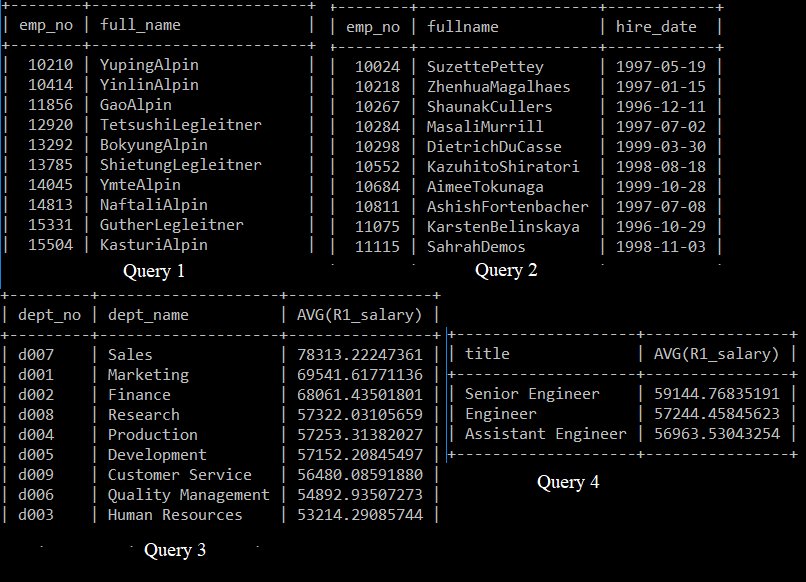
\includegraphics[scale = 0.8]{result.PNG}
\caption{Results}
\end{figure}
\end{document}
